\section{Interaktion zwischen Skill und Objekt} \label{SkillObjektInteraktion}
	Anhand eines Beispiels (\ref{fig:Skillinteraktion}) soll die Interaktion zwischen einem Skill und den zugehörigen Objekten erläutert werden. Der Skill «\verb|Skill_P2P|» ermöglicht es einem Roboter, zu einem definierten Punkt zu fahren. Falls der Roboter dabei mit einem Hindernis kollidiert, wird der Roboter durch den Skill gestoppt. Hindernisse werden dabei mithilfe eines Kraftsensors erkannt.
	\\
	Der Skill wird über Eingangsvariablen mit den entsprechenden Objekten verbunden, was durch eine blaue Verbindungslinie dargestellt wird. Über die Sequenz werden verschiedene Informationen an den Skill übergeben. Dazu zählen:
	\begin{itemize}
		\item Die aktuelle Position des Roboters
		\item Die Geschwindigkeit und Beschleunigung
		\item Die Art der Bewegung bzw. Positionierung
		\item Die Kraftgrenze, die ein Hindernis definiert
	\end{itemize}
	
	Der Start des Skills erfolgt durch die Start-Methode, die von der Sequenz ausgelöst wird. Der Skill selbst initiiert über die Start-Methode des Aktor-Objekts den Bewegungsprozess und liest parallel dazu mithilfe der Messdaten-Eigenschaft die Daten des Sensor-Objekts aus. Die Objekte haben dabei ausschliesslich der Aufgabe, ihre spezifischen Funktionen auszuführen, die durch ihre jeweilige Komponente definiert sind. Sie enthalten keine Logik in Bezug auf das Gesamtsystem – diese liegt vollständig im Skill.
	\\
	Der Skill analysiert die übermittelten Daten und reagiert entsprechend darauf. Im geschilderten Beispiel stoppt der Skill den Aktor, sobald die gemessenen Daten die vorgegebenen Schwellenwerte überschreiten.
	
	\begin{figure}[h!]
		\centering
		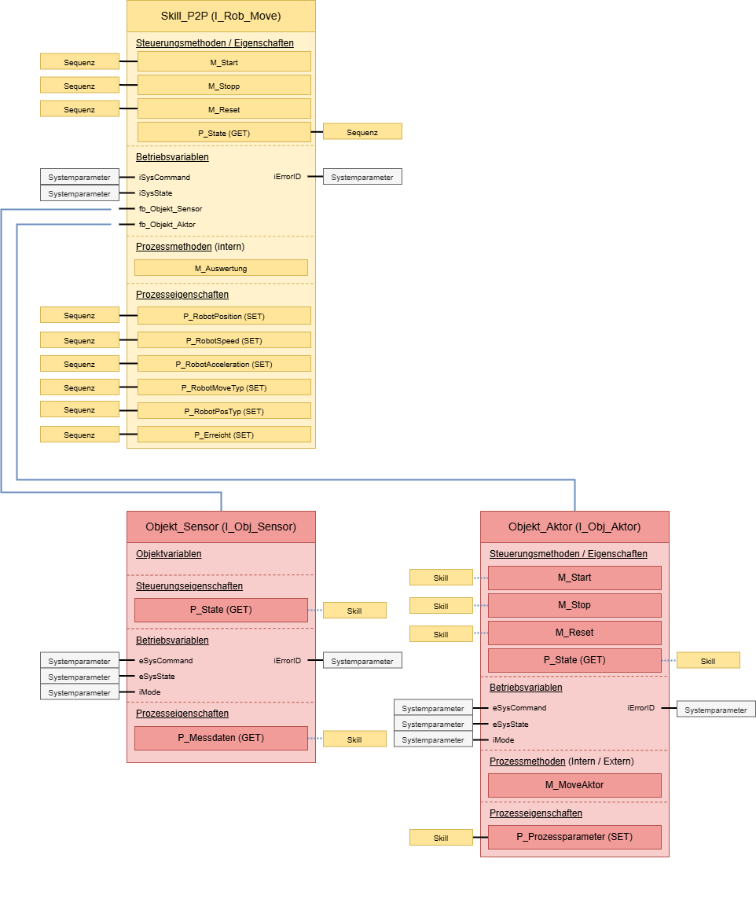
\includegraphics[width=1\textwidth]{06_Skillentwicklung/Skillinteraktion}
		\captionsetup{justification=centering}
		\caption{Skill-Interaktion}
		\label{fig:Skillinteraktion}
	\end{figure}
	
	\newpage
	
	
	